% SC2203 --- Chapter 4: Context-Free Grammars and Languages (0->100 ground-up)
\chapter{Context-Free Grammars and Languages}
\label{ch:contextfree}

\begin{quote}
\emph{``Regular languages cannot count.''} --- To capture $0^n1^n$ and nesting (parentheses, \texttt{if--else}), we add recursion: grammars whose rules expand a variable into strings of variables and terminals.
\end{quote}

\noindent\fbox{\parbox{\dimexpr\linewidth-2\fboxsep-2\fboxrule}{%
\textbf{From zero: we build here, no grammar assumed.} We define CFG from scratch---terminals, variables, productions, derivations---with trees before formalism. Induction on derivations proves language membership. Only Ch.~1--2 required.}}
\vspace{0.4em}

\section*{Learning Outcomes}
After this chapter you will be able to:
\begin{enumerate}[label=(L\arabic*)]
    \item define CFG, derivation, parse tree and language $L(G)$;
    \item design CFGs for counting and nesting languages ($0^n1^n$, palindromes, $a^nb^m$);
    \item determine ambiguity and eliminate it where possible (or prove inherent);
    \item convert a CFG to Chomsky normal form (CNF) with proof sketch;
    \item state and apply the pumping lemma for CFLs to show non-context-freeness.
\end{enumerate}

% ============================================================
\section{Context-Free Grammars}
\label{sec:cfg-def}
\emph{Intuition:} a variable is a placeholder for a language; a rule $A\to\alpha$ says ``replace $A$ by $\alpha$''. Starting from $S$, repeatedly replace until only terminals remain.

\begin{definition}[CFG]
A \emph{context-free grammar} is $G=(V,\Sigma,R,S)$ where $V$ variables, $\Sigma$ terminals ($\Sigma\cap V=\emptyset$), $R\subseteq V\times(V\cup\Sigma)^*$ finite productions $A\to\alpha$, $S\in V$ start. Write $\Rightarrow$ for one-step derivation ($\beta A\gamma\Rightarrow\beta\alpha\gamma$ if $A\to\alpha$), $\Rightarrow^*$ for zero-or-more steps. $L(G)=\{w\in\Sigma^*\mid S\Rightarrow^*w\}$.
\end{definition}

\begin{example}[The canonical $0^n1^n$]
$G$: $S\to0S1\mid\varepsilon$. Derivation of $0011$: $S\Rightarrow0S1\Rightarrow00S11\Rightarrow0011$. Language is $\{0^n1^n\mid n\ge0\}$---proved by induction: $S\Rightarrow^*0^n1^n$ for all $n$ (induction on $n$), and no other strings derivable (induction on derivation length; the first rule applied determines the outer $0/1$ pair).
\end{example}

\begin{example}[Palindromes and nesting]
Over $\{0,1\}$: $P\to0P0\mid1P1\mid0\mid1\mid\varepsilon$ generates all palindromes. For balanced parentheses with $\Sigma=\{(,)\}$: $S\to SS\mid(S)\mid\varepsilon$. For $a^ib^jc^k$ with $i=j$ or $j=k$ variations, we branch at the top: $S\to AB\mid CD$ with separate sub-grammars---union via new start.
\end{example}

% TikZ 1: derivation tree for 0^n1^n
\begin{figure}[h]
\centering
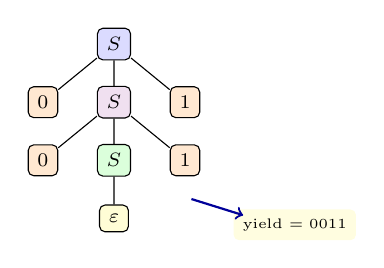
\begin{tikzpicture}[scale=0.82,level distance=9mm,sibling distance=11mm,every node/.style={font=\scriptsize}]
\node[draw,fill=blue!14,rounded corners=2pt] {$S$}
  child {node[fill=orange!18,rounded corners=2pt,draw] {$0$}}
  child {node[draw,fill=violet!12,rounded corners=2pt] {$S$}
    child {node[fill=orange!18,draw,rounded corners=2pt] {$0$}}
    child {node[draw,fill=green!14,rounded corners=2pt] {$S$}
      child {node[fill=yellow!16,draw,rounded corners=2pt] {$\varepsilon$}}
    }
    child {node[fill=orange!18,draw,rounded corners=2pt] {$1$}}
  }
  child {node[fill=orange!18,draw,rounded corners=2pt] {$1$}};
\node[font=\tiny,fill=yellow!12,rounded corners=2pt] at (2.8,-2.8) {yield $=0011$};
\draw[->,thick,blue!60!black] (1.2,-2.4)--(2.0,-2.65);
\end{tikzpicture}
\caption{Parse tree for $0011$ via $S\to0S1$: recursion nests; frontier (leaves left-to-right) is the derived string. Every derivation corresponds to a tree.}
\label{fig:parse-tree-0n1n}
\end{figure}

\begin{definition}[Parse tree, leftmost derivation]
A \emph{parse tree} has root $S$, interior nodes in $V$, leaves in $\Sigma\cup\{\varepsilon\}$, and children of $A$ spell a production $A\to\alpha$. Yield = concatenation of leaves. A \emph{leftmost} derivation always expands the leftmost variable; it traces a depth-first traversal.
\end{definition}

% TikZ 2: ambiguity example (if-else dangling)
\begin{figure}[h]
\centering
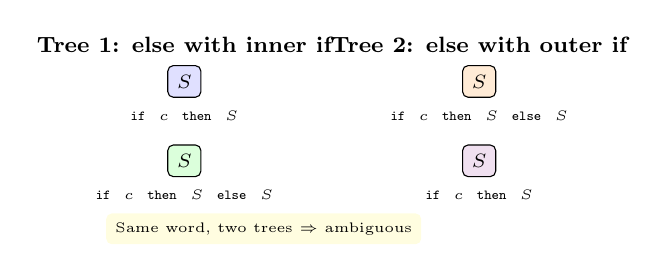
\begin{tikzpicture}[scale=0.72,every node/.style={font=\scriptsize}]
\begin{scope}
\node[font=\footnotesize\bfseries] at (1.2,1.5) {Tree 1: else with inner if};
\node[draw,fill=blue!12,rounded corners=2pt] at (1.2,0.85) {$S$};
\node[font=\tiny] at (1.2,0.25) {\texttt{if } $c$ \texttt{ then } $S$};
\node[draw,fill=green!14,rounded corners=2pt] at (1.2,-0.55) {$S$};
\node[font=\tiny] at (1.2,-1.15) {\texttt{if } $c$ \texttt{ then } $S$ \texttt{ else } $S$};
\end{scope}
\begin{scope}[xshift=5.2cm]
\node[font=\footnotesize\bfseries] at (1.2,1.5) {Tree 2: else with outer if};
\node[draw,fill=orange!16,rounded corners=2pt] at (1.2,0.85) {$S$};
\node[font=\tiny] at (1.2,0.25) {\texttt{if } $c$ \texttt{ then } $S$ \texttt{ else } $S$};
\node[draw,fill=violet!12,rounded corners=2pt] at (1.2,-0.55) {$S$};
\node[font=\tiny] at (1.2,-1.15) {\texttt{if } $c$ \texttt{ then } $S$};
\end{scope}
\node[font=\tiny,fill=yellow!12,rounded corners=2pt] at (2.6,-1.75) {Same word, two trees $\Rightarrow$ ambiguous};
\end{tikzpicture}
\caption{The dangling-else ambiguity: one string, two parse trees. Real languages fix this by grammar refactoring or precedence declarations.}
\label{fig:ambiguity-ifelse}
\end{figure}

\begin{definition}[Ambiguity]
$G$ is \emph{ambiguous} if some $w\in L(G)$ has two distinct parse trees (equivalently two leftmost derivations). $L$ is \emph{inherently ambiguous} if every CFG for $L$ is ambiguous (e.g.\ $\{a^ib^jc^k\mid i=j\text{ or }j=k\}$).
\end{definition}

\begin{example}[Proving $L(G)=\{0^n1^n\}$ by induction]
We show $S\Rightarrow^*0^n1^n$ by induction on $n$ (base $\varepsilon$, step via $S\to0S1$). Conversely, if $S\Rightarrow^*w$, induction on derivation length: first step must be $S\Rightarrow0S1\Rightarrow^*w$, so $w=0x1$ with shorter derivation $S\Rightarrow^*x$; by IH $x=0^{n-1}1^{n-1}$, hence $w=0^n1^n$. This two-direction induction is the template for all CFG correctness proofs.
\end{example}

\begin{remark}[Design pattern]
For union $L_1\cup L_2$, new $S\to S_1\mid S_2$; for concat $S\to S_1S_2$; for star $S\to SS_1\mid\varepsilon$. These combinators mirror regex operators and preserve context-freeness directly via grammar surgery.
\end{remark}

% ============================================================
\section{Chomsky Normal Form}
\label{sec:cnf}
CNF restricts productions to $A\to BC$ or $A\to a$ (plus $S\to\varepsilon$ if needed), enabling $O(n^3)$ parsing (CYK) and pumping proofs.

\begin{theorem}[CNF conversion]
For every CFG $G$ there is $G'$ in CNF with $L(G')=L(G)\setminus\{\varepsilon\}$ (and $S\to\varepsilon$ added iff $\varepsilon\in L(G)$). Transformation is effective: eliminate $\varepsilon$-productions, unit productions, and long right-hand sides.
\end{theorem}
\begin{proof}[Sketch]
\emph{1. Nullable:} compute $A$ with $A\Rightarrow^*\varepsilon$ (fixed point), add all $\varepsilon$-free variants of each production (if $A\to BCD$ with $C$ nullable, add $A\to BD$ etc.). Remove $A\to\varepsilon$ except possibly $S\to\varepsilon$. \emph{2. Units:} if $A\stackrel{*}{\Rightarrow}B$ via $A\to B$, replace $A\to B$ by $A\to\alpha$ for each $B\to\alpha$ non-unit. \emph{3. Long:} replace $A\to X_1\cdots X_k$ ($k\ge3$) by $A\to X_1Y_1$, $Y_1\to X_2Y_2$, \dots; replace terminals $a$ in long bodies by new $T_a\to a$. Each step preserves language. \qed
\end{proof}

\begin{example}[CNF trace]
$G$: $S\to aSb\mid SS\mid\varepsilon$ (balanced $a^nb^n$ concatenations). Nullable = $\{S\}$. After step~1: $S\to aSb\mid ab\mid SS\mid S\mid\varepsilon$; step~2 removes $S\to S$; step~3 breaks $aSb$ into $S\to AT$, $T\to SB$, $A\to a$, $B\to b$. Result has $\le2$ symbols per body. CYK can now parse $ab$ via $A B$.
\end{example}

\begin{example}[Why CNF matters for complexity]
Without CNF, a production $A\to B C D E$ could be arbitrarily long, but CNF's binary form bounds branching. Hence any $w$ with $|w|=n$ has a parse tree with $2n-1$ internal nodes (exactly), giving the $2^{|V|}$ pumping bound and the $O(n^3)$ CYK table size---both impossible without length restriction.
\end{example}

% TikZ 3: CNF binary tree shape
\begin{figure}[h]
\centering
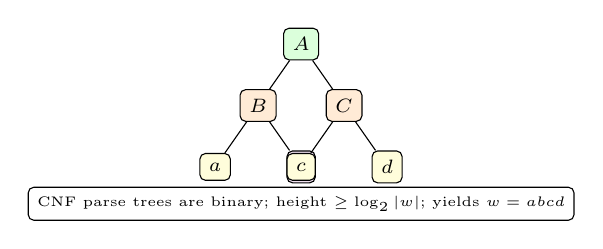
\begin{tikzpicture}[scale=0.78,level distance=10mm,sibling distance=14mm,every node/.style={font=\scriptsize,draw,rounded corners=2pt,fill=blue!10}]
\node[fill=green!14] {$A$}
  child {node[fill=orange!16] {$B$}
    child {node[fill=yellow!14] {$a$}}
    child {node[fill=violet!12] {$b$}}
  }
  child {node[fill=orange!16] {$C$}
    child {node[fill=yellow!14] {$c$}}
    child {node[fill=yellow!14] {$d$}}
  };
\node[font=\tiny,fill=white] at (0,-2.6) {CNF parse trees are binary; height $\ge\log_2|w|$; yields $w=abcd$};
\end{tikzpicture}
\caption{In CNF every internal node has exactly two variable children or one terminal; parse trees are binary, so long words force a tall branch that will repeat a variable.}
\label{fig:cnf-binary}
\end{figure}

% ============================================================
\section{Pumping Lemma for CFLs}
\label{sec:pumping-cfl}
Idea: tall CNF tree for long $w$ has a root-to-leaf path with repeated variable $A$ (pigeonhole on $|V|$); the subtree rooted at the higher $A$ can be pumped.

\begin{theorem}[Pumping lemma, CFL]
If $L$ CFL then $\exists p\ge1$ (here $p=2^{|V|}$) such that $\forall w\in L$, $|w|\ge p$, $\exists$ split $w=uvxyz$ with (i) $|vxy|\le p$, (ii) $|vy|>0$, (iii) $\forall i\ge0:\;uv^ixy^iz\in L$.
\end{theorem}
\begin{proof}[Sketch]
Take CNF $G$ for $L\setminus\{\varepsilon\}$. For $|w|\ge2^{|V|}$, any parse tree has height $\ge|V|+1$, so some variable $A$ repeats on a leaf-to-root path. Let upper $A\Rightarrow^*vAy$ (with $v,y$ possibly empty but not both) and $A\Rightarrow^*x$. Then $S\Rightarrow^*uAy\Rightarrow^*uvA y z\Rightarrow^*uvxyz$ and iterating the $A$-loop gives $uv^ixy^iz$. Bound $|vxy|\le2^{|V|}=p$ because the subtree depth at the repeat is $\le|V|+1$. \qed
\end{proof}

\begin{example}[Showing $\{a^nb^nc^n\mid n\ge0\}$ not CFL]
Assume CFL with $p$. Take $w=a^pb^pc^p$. Any split $uvxyz$ with $|vxy|\le p$ touches at most two of the three blocks (pigeonhole on blocks). If $vxy$ lies in $a$'s and $b$'s, pumping changes $a$'s or $b$'s but not $c$'s, breaking $n$-equality. Formal: if $v$ or $y$ contains mixed symbols $a$ and $b$, $uv^2xy^2z$ has shape violation $a^*b^*a^*...$; else pumping unbalances counts. Hence not CFL. By closure, $\{a^nb^nc^n\}$ separates CFL from regular.
\end{example}

\begin{example}[When pumping fails but $L$ still not CFL]
$L=\{a^ib^jc^k\mid i\le j\le k\}$ is not CFL but pumping alone needs care because $|vxy|\le p$ can be placed to pump within one block while preserving $i\le j\le k$. Instead use Ogden's lemma (marked positions) or closure: intersect with $a^*b^*c^*$ and use stronger condition. This mirrors the regular case where pumping is necessary but not sufficient.
\end{example}

\begin{remark}[Pumping game for CFLs]
As with regular pumping, the CFL game is: adversary picks $p$, you pick $w$, adversary splits $w=uvxyz$, you pump. The bound $|vxy|\le p$ is the new weapon---it forces $vxy$ to be local, so a clever $w=a^pb^pc^p$ spreads over three blocks and any local $vxy$ misses one block. Choose $w$ to maximise this locality trap.
\end{remark}

% ============================================================
\section{Closure Properties of CFLs}
\label{sec:cfl-closure}
CFLs are closed under $\cup$, concat, $*$, substitution, homomorphism, inverse homomorphism, reversal, but \emph{not} under $\cap$ or complement. Example: $L_1=\{a^nb^nc^m\}$, $L_2=\{a^mb^nc^n\}$ are CFL, but $L_1\cap L_2=\{a^nb^nc^n\}$ is not. Hence $\overline{L_1}$ cannot be CFL (otherwise $\cap$ would be via De Morgan and $\cup$).
Intersection with a \emph{regular} language \emph{does} stay CFL (product of PDA and DFA in Ch.~5), a useful tool: intersect suspected non-CFL with $a^*b^*c^*$ to isolate the hard core before pumping.

\begin{example}[CYK preview on CNF]
CYK parses $w=a_1\cdots a_n$ by DP: $T[i,j]=\{A\mid A\Rightarrow^* a_i\cdots a_j\}$. Initialise $T[i,i]=\{A\mid A\to a_i\}$; then $T[i,j]=\bigcup_{k}\{A\mid A\to BC,\;B\in T[i,k],\,C\in T[k+1,j]\}$. Accept iff $S\in T[1,n]$. For $w=ab$ with CNF above, $T[1,1]=\{A\}$, $T[2,2]=\{B\}$, $T[1,2]$ contains $S$ via $S\to AB$---$O(n^3|G|)$.
\end{example}

\begin{theorem}[Decidability for CFLs]
Emptiness ($L(G)=\emptyset$?), finiteness, and membership ($w\in L(G)$?) are decidable (reachability on variables and CYK). Universality, equivalence, inclusion, and regularity of a CFL are undecidable (reduce from halting via Ch.~7).
Membership via CYK is $O(n^3|G|)$ in CNF; emptiness is linear by marking reachable variables---graph reachability again.
Finiteness is also decidable: check for a pumpable variable that derives itself with non-trivial yield and is reachable from $S$ and can derive a terminal string.
\end{theorem}

% ============================================================
\section{Chapter Notes}
Chomsky (1956) introduced CFGs and CNF; Bar-Hillel's CFL pumping (1961) and later Ogden (1968) refined non-membership proofs. CYK parsing ($O(n^3|G|)$) follows from CNF's binary shape and is used in Ch.~5 for PDA equivalence. Inherent ambiguity was shown by Parikh for $\{a^ib^jc^k\mid i=j\text{ or }j=k\}$.
Greibach normal form ($A\to a\alpha$, $\alpha\in V^*$) is an alternative that yields top-down parsing and connects to PDAs in Ch.~5.
For compilers, LL/LR subsets of CFGs suffice for deterministic parsing; the general CFG problem is $O(n^3)$.
The pumping bound $p=2^{|V|}$ is tight: the language $\{a^{2^{n}}\}$ needs that many variables in CNF to force a repeat, illustrating exponential succinctness gaps between grammars.

% ============================================================
\section{Exercises}
\label{sec:ch04-exercises}
Each exercise reinforces the grammar $\leftrightarrow$ tree $\leftrightarrow$ CNF $\leftrightarrow$ pumping cycle.
Exercises E4.4--E4.5 use Ogden or closure with $a^*b^*c^*$ to avoid case analysis traps.
\begin{enumerate}[label=E4.\arabic*, leftmargin=*, itemsep=0.8em]
\item \textbf{Grammar design.} Give CFG for $L=\{0^i1^j\mid i\le j\}$ and for $L=\{w\mid w$ has more $0$s than $1$s$\}$. Prove correctness by induction on derivations for one of them.
\item \textbf{Ambiguity test.} Is $S\to S+S\mid S*S\mid(S)\mid a$ ambiguous? Exhibit two trees for $a+a*a$, then refactor with precedence layers $E\to E+T\mid T$, $T\to T*F\mid F$, $F\to(E)\mid a$ and argue unambiguous.
\item \textbf{CNF conversion.} Convert $S\to aS b\mid S S\mid\varepsilon$ to CNF step by step: list nullable, eliminate $\varepsilon$, eliminate units, break long bodies. Show parse of $aabb$ in CNF.
\item \textbf{CFL pumping.} Use pumping to prove $\{a^n b^n c^n\mid n\ge0\}$ not CFL; consider cases where $vxy$ straddles blocks vs.\ lies inside one block, and why $|vxy|\le p$ forces at most two blocks.
\item \textbf{Non-closure.} Prove CFLs not closed under intersection via $L_1=\{a^nb^nc^m\}$ and $L_2=\{a^mb^nc^n\}$; deduce non-closure under complement. Give closure under union/concat/$*$ by construction on grammars.
\item \textbf{Bonus: Ogden.} State Ogden's lemma (marked positions) and use it to show $\{a^ib^jc^k\mid i\le j\le k\}$ not CFL more cleanly.
\end{enumerate}
% End of Chapter 4
